\chapter{Resultados}

\section{Búsqueda y Selección}
    \subsection{Caso promedio}
        \subsubsection{Búsqueda}
        \begin{figure}[H]
            \centering
            
\includegraphics[width=1\textwidth]{./Fig/search_average_benchmark.pdf}
            \caption{Comparación de tiempos en el caso promedio}\label{fig:average_case_search}
        \end{figure}

        \subsubsection{Sorting}
        \begin{figure}[H]
            \centering
            
\includegraphics[width=1\textwidth]{./Fig/sort_average_benchmark.pdf}
            \caption{Comparación de tiempos en el caso promedio}\label{fig:average_case_sort}
        \end{figure}
        \begin{figure}[H]
            \centering
            \includegraphics[width=1\textwidth]{./Fig/sort_average_benchmark_dyv.pdf}
            \caption{Comparación de tiempos en el caso promedio en Divide y Vencerás}\label{fig:average_case_sort_dyv}
        \end{figure}
    \subsection{Mejor caso}
        \subsubsection{Sorting}
            \begin{figure}[H]
                \centering
                
\includegraphics[width=1\textwidth]{./Fig/sort_best_benchmark.pdf}
                \caption{Comparación de tiempos en el mejor caso}\label{fig:best_case_sort}
            \end{figure}

            \begin{figure}[H]
                \centering
                \includegraphics[width=1\textwidth]{./Fig/sort_best_benchmark_dyv.pdf}
                \caption{Comparación de tiempos en el mejor caso en Divide y Vencerás}\label{fig:best_case_sort_dyv}
            \end{figure}

    \subsection{Peor caso}
        \subsubsection{Sorting}
            \begin{figure}[H]
                \centering
                
\includegraphics[width=1\textwidth]{./Fig/sort_worst_benchmark.pdf}
                \caption{Comparación de tiempos en el peor caso}\label{fig:worst_case_sort}
            \end{figure}

            \begin{figure}[H]
                \centering
                \includegraphics[width=1\textwidth]{./Fig/sort_worst_benchmark_dyv.pdf}
                \caption{Comparación de tiempos en el peor caso en Divide y Vencerás}\label{fig:worst_case_sort_dyv}
            \end{figure}
        \subsubsection{Search}
            \begin{figure}[H]
                \centering
                
\includegraphics[width=1\textwidth]{./Fig/search_worst_benchmark.pdf}
                \caption{Comparación de tiempos en el peor caso}\label{fig:worst_case_search}
            \end{figure}

\section{Selección (Quickselect)}
            \begin{figure}[H]
                \centering
                
\includegraphics[width=1\textwidth]{./Fig/selection_benchmark.pdf}
                \caption{Comparación de tiempos en selección}\label{fig:selection_benchmark}
            \end{figure}

\section{Threshold}
    \begin{figure}[H]
        \centering
        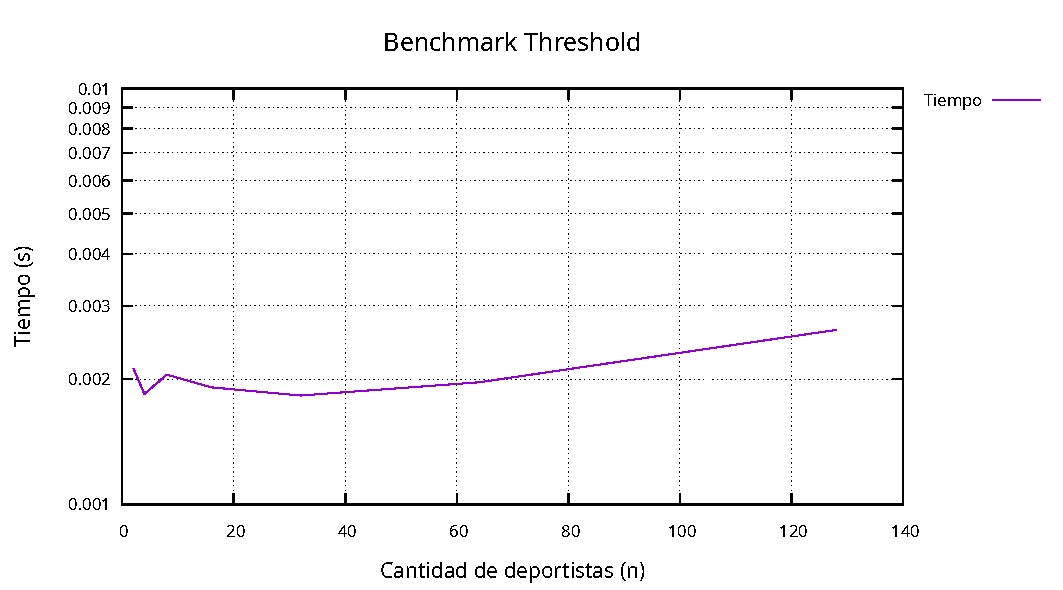
\includegraphics[width=0.8\textwidth]{./Fig/threshold_benchmark.pdf}
        \caption{Benchmark de threshold}
        \label{fig:threshold_benchmark}
    \end{figure}

\chapter{Análisis de resultados}

\section{Ordenamiento}
En el caso promedio y peor, los algoritmos Merge Sort y Quick Sort mantienen tiempos de ejecución significativamente menores a los algoritmos iterativos, como lo son Bubble Sort o Selection Sort. 
Entre estos, Merge Sort se muestra como el de mayor estabilidad tanto en su versión estándar como en su versión optimizada, sus tiempos de ejecución se mantienen consistentes en todos los casos. La versión optimizada de Merge Sort presenta una mejora ligera pero constante en el tiempo de procesamiento en todas las pruebas.

Por otro lado, Quick Sort muestra una variabilidad crítica dependiente de la elección del pivote. En las variantes de pivote fijo (\textit{first} y \textit{last}), el algoritmo sufre una degradación de complejidad hacia $O(n^2)$ cuando los datos están ya ordenados o inversamente ordenados. Sin embargo, las implementaciones con pivote aleatorio (\textit{random}) o mediana de tres (\textit{median}) corrigen esta inestabilidad, manteniendo el comportamiento $O(n \log n)$ incluso en los peores escenarios.

\section{Búsqueda y Selección}
La Búsqueda Binaria (iterativa y recursiva) y la Exponencial, demuestran una alta eficiencia logarítmica. En los benchmarks de caso promedio y peor, estos algoritmos mantienen tiempos de ejecución extremadamente bajos, validando su superioridad frente a la búsqueda secuencial. No se observa una penalización significativa por el uso de recursión en la búsqueda binaria en comparación con su contraparte iterativa.

Respecto a la selección, el algoritmo Quickselect muestra un crecimiento de tiempo que tiende a la linealidad. Al igual que Quick Sort, presenta una brecha visible entre el mejor y peor caso.

\section{Optimización mediante Umbral (Threshold)}
El mejor tiempo promedio se consiguió con un umbral de aproximadamente 32 elementos (tiempo medido: 0.001826 s). Esto significa que, si el umbral es muy pequeño (ej. 2 u 8), el programa hace demasiadas llamadas recursivas y pierde tiempo en la sobrecarga de la función. Si el umbral es muy grande (ej. 128), se hace demasiado trabajo localmente al usar el algoritmo simple, y también se pierde rendimiento.

Por lo tanto, el umbral óptimo es un equilibrio entre la profundidad de la recursión y la eficiencia del algoritmo simple utilizado para ordenar los subproblemas pequeños. Por ejemplo un umbral de 32 parece ser un punto adecuado que minimiza el tiempo total de ejecución.
